\documentclass[12pt,aspectratio=169]{beamer}

\usetheme{metropolis}

\definecolor{mDarkBrown}{HTML}{FF5722}
\definecolor{mDarkTeal}{HTML}{263238}
\definecolor{mLightBrown}{HTML}{FF5722}

\usepackage{booktabs}
\usepackage{graphicx}
\usepackage{hyphenat}
\usepackage{multirow}
\usepackage{nicefrac}
\usepackage[normalem]{ulem}

\usepackage{pifont}
\newcommand{\cmark}{\ding{51}}
\newcommand{\xmark}{\ding{55}}

\usepackage{minted}
\usemintedstyle{tango}
\newminted[bash]{bash}{%
    autogobble,
    bgcolor=mDarkTeal!10,
    linenos
}
\newminted[py3]{python}{%
    python3,
    autogobble,
    bgcolor=mDarkTeal!10,
    linenos
}
\newminted[sql]{sql}{%
    autogobble,
    bgcolor=mDarkTeal!10,
    linenos
}

\usepackage{polyglossia}
\setdefaultlanguage[variant=british]{english}
\usepackage[english=british]{csquotes}

\defaultfontfeatures{Ligatures=TeX}
\setmainfont{Lucida Sans OT}
\setsansfont[Scale=MatchLowercase]{Lucida Sans OT}
\setmonofont[Scale=MatchLowercase]{Lucida Console DK}

\usepackage{mathspec}
\setmathsfont(Digits,Latin,Greek)[Numbers={Lining,Proportional}]{Lucida Bright Math OT}

\newcommand{\mat}[1]{\ensuremath{\mathbf{#1}}}

\newcommand{\R}{\ensuremath{\mathbb{R}}}

\newcommand{\E}[1]{\ensuremath{\mathbb{E}\!\left[ #1 \right]}}
\newcommand{\V}[1]{\ensuremath{\mathbb{V}\!\left[ #1 \right]}}
\newcommand{\Prob}[1]{\ensuremath{\Pr\!\left( #1 \right)}}
\newcommand{\Normal}[2]{\ensuremath{\mathcal{N}\!\left( #1, #2 \right)}}
\newcommand{\simiid}{\ensuremath{\overset{\text{\tiny i.i.d.}}{\sim}}}

\DeclareMathOperator{\logit}{logit}

\author{Gianluca Campanella}
\date{}



\title{Support vector machines}

\begin{document}

\maketitle

\begin{frame}{Support vectors}
    \begin{center}
        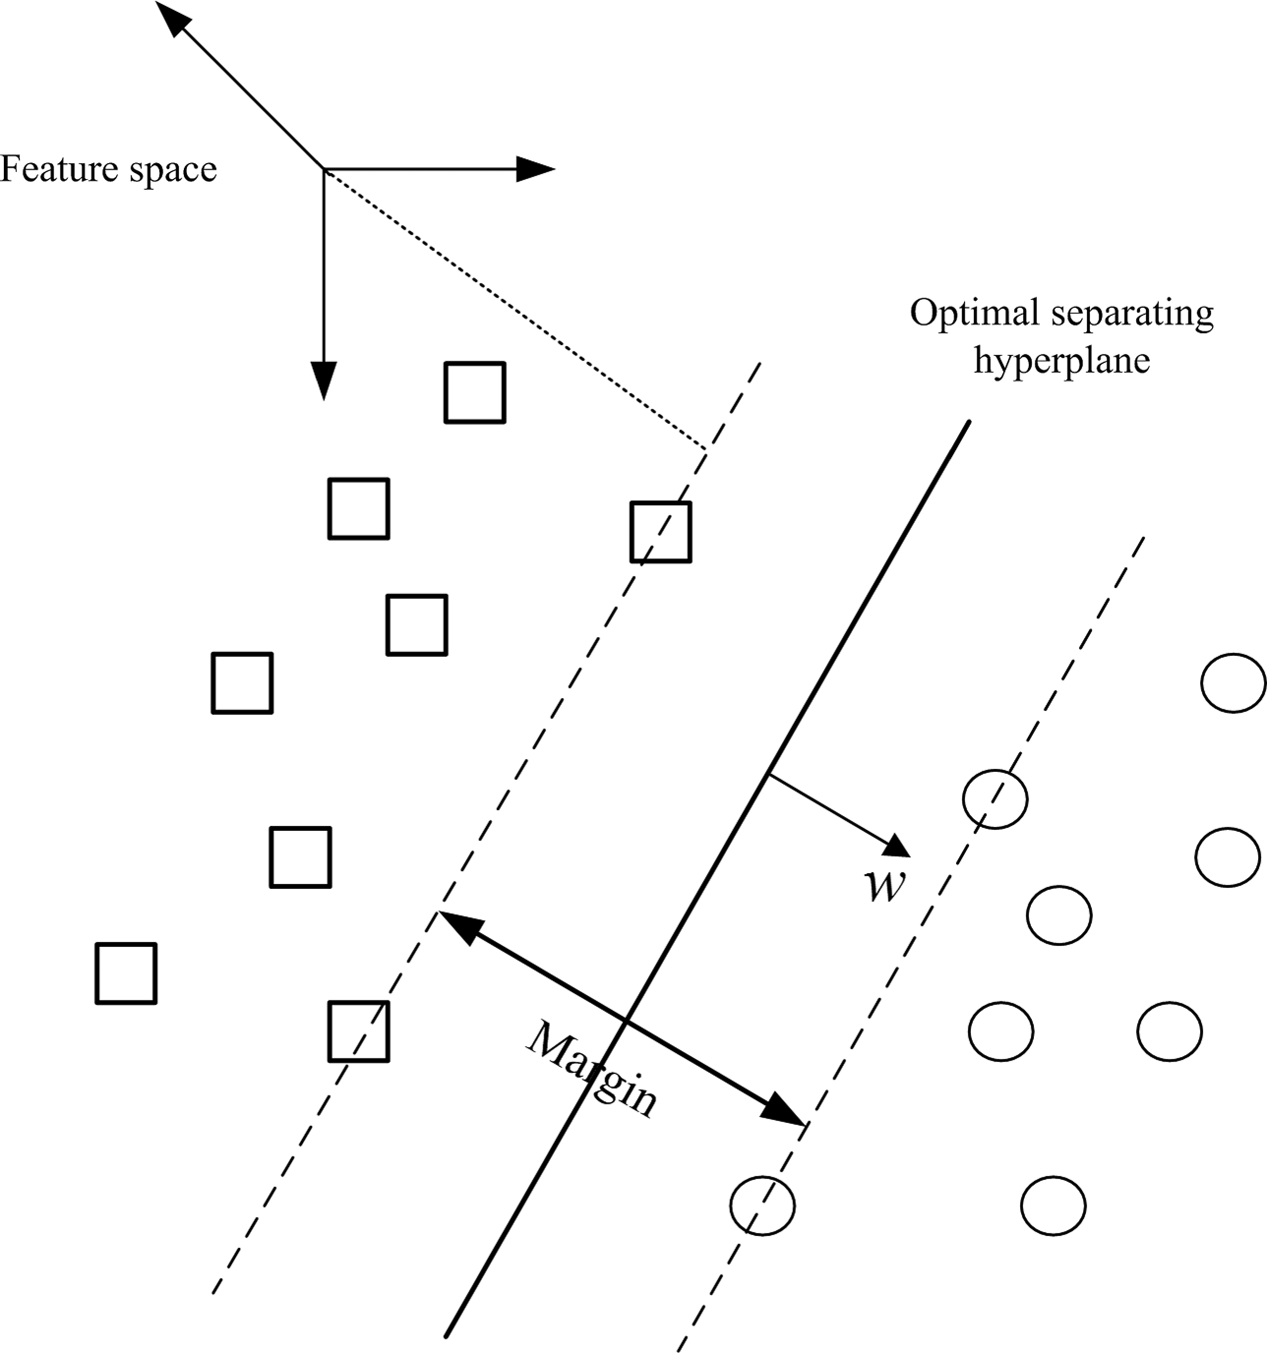
\includegraphics[height=0.8\textheight]{figures/support_vectors} \\
        {\scriptsize%
         From Li et al.\ (2011)}
    \end{center}
\end{frame}

\begin{frame}{Margin}
    \only<1>{%
        \begin{center}
            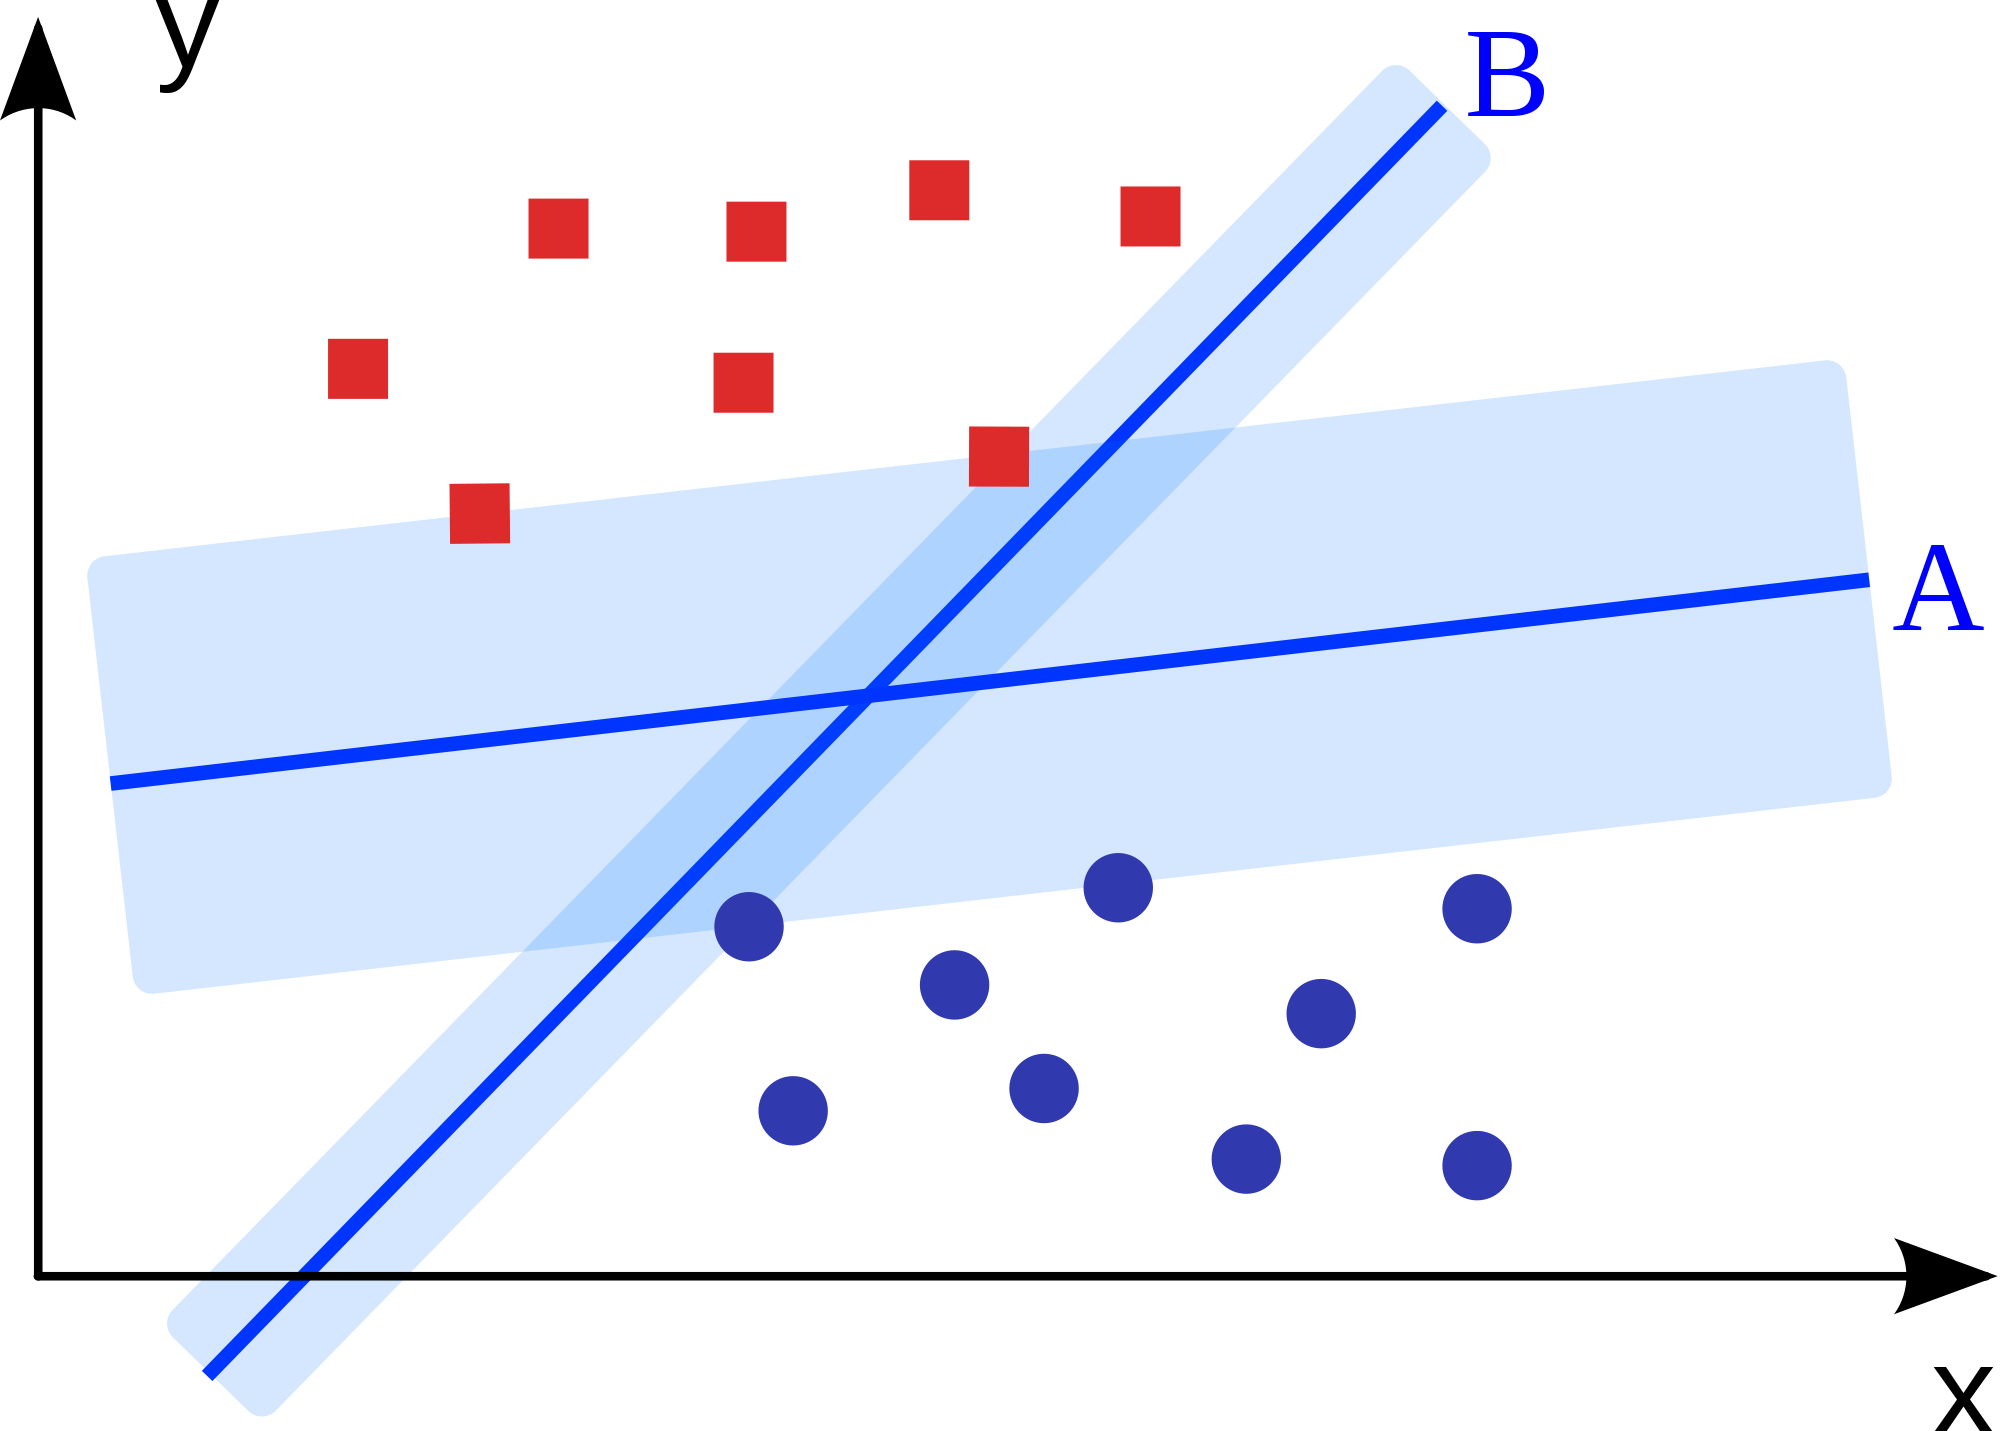
\includegraphics[height=0.8\textheight]{figures/margin} \\
            {\scriptsize%
             Via \textit{Wikimedia Commons}}
        \end{center}}
    \only<2>{%
        \begin{itemize}
            \item \alert{Maximising the margin is good}
            \item[$\rightarrow$] Less overfitting
            \item[$\rightarrow$] Model generalises better \\[\bigskipamount]
            \item Only support vectors are important \\[\bigskipamount]
            \item Can be done by solving a quadratic optimisation problem
                  subject to linear constraints
        \end{itemize}}
\end{frame}

\begin{frame}{Hard and soft\hyp{}margin SVM}
    \begin{block}{Hard\hyp{}margin}
        \begin{itemize}
            \item Requires correct classification of \alert{all} samples
            \item Only solvable if samples are linearly separable
        \end{itemize}
    \end{block}
    \vfill\pause
    \begin{block}{Soft\hyp{}margin}
        \begin{itemize}
            \item \alert{Some} misclassification is allowed
            \item Will `compromise' on model performance to obtain a larger
                  margin $\rightarrow$ more generalisable model
        \end{itemize}
    \end{block}
\end{frame}

\begin{frame}{Non\hyp{}linear SVM}
    \begin{block}{Idea}
        Map the original input space to some higher\hyp{}dimensional space
        where the training set is linearly separable
    \end{block}
    \vfill
    \begin{block}{`Kernel trick'}
        \begin{itemize}
            \item Effectively introduces new predictors
            \item \alert{No need to compute (and store) the expanded dataset}
        \end{itemize}
    \end{block}
\end{frame}

\begin{frame}{Pros and cons}
    \begin{block}{Pros}
        \begin{itemize}
            \item Can handle large datasets (only support vectors matter)
            \item Effective in high\hyp{}dimensional spaces ($p > n$)
            \item Mathematically `convenient' (also `kernel trick')
        \end{itemize}
    \end{block}
    \vfill
    \begin{block}{Cons}
        \begin{itemize}
            \item Prone to overfitting ($\rightarrow$ use soft\hyp{}margin)
            \item Do not provide probability estimates directly
        \end{itemize}
    \end{block}
\end{frame}

\end{document}

